\chapter{Technical design}
\label{chap:technical-design}
% repeat technical specifics of the architecture - choice of languages, frameworks, libraries and other tools
The large number of options from spectre of  programming languages and associated frameworks presents both an opportunity and a challenge at the same time in today's fast paced technological landscape.
As we move into the technical details of the architecture presented in the previous chapter \ref{chap:architectural-design}, it is important to recall an idea mentioned in \cite{sommervilleSW}. Establishing a robust architecture in the early stages of development is key because it will become significantly more expensive in future phases than at the beginning. 
These phases and decisions are very closely linked. 
Because, as important as how we lay out the application, it is equally important how and with what we write it.

In this chapter, we examine the technical decisions that shape the development and operation of the platform.
We will explore the selection of programming languages and frameworks, detailing how these choices work together to create a robust, scalable foundation for the system.
Additionally, this chapter will address an approach to a multi-tenancy design paradigm - a key architectural feature that enables us to efficiently manage resources and serve multiple clients within a single application instance.
Now, with an added layer of detail regarding the programming languages, frameworks, and technologies, this architecture can be brought to life. 

\section{Programming Language and Frameworks}
\label{sec:programming-language-frameworks}
% introduction to the importance of choosing programming lang + framework
% stating primary choices: TS, React, Koa, PSQL
Choosing the right programming language and frameworks is a crucial decision that influences not only the development process but also the longevity of the software itself.
Impacts every phase of the development life-cycle, from initial implementation to maintenance and the capacity to scale in response to future demands.
In the following section, the platform technology stack will be presented with the reasoning behind these decisions and the alternatives taken into consideration. 

The core technologies that form the backbone of the platform include TypeScript for programming, React for the frontend development, Koa as the backend framework and PostgreSQL for data management.
Let us dive into more detail and reasoning behind these decisions.

\subsection{Programming Language}
\label{subsec:programming-language}
% why TS, compare maybe with python
In the world of full-stack web development, TypeScript has evolved as a popular choice for both frontend and backend development, largely due to its widespread and support from community.
The decision to use TypeScript across the entire stack is aligned with the project's goals of scalability, maintainability, and productivity.

When discussing TypeScript, it is, of course, fair to mention JavaScript, the (almost) native language of the Web.
However, JavaScript is a subset of TypeScript for some reason.
Static Type Checking with TypeScript offers significant advantages in terms of code quality and reliability.
It makes TypeScript a more verbose and complex language to write, but in the long run and in such a large project it helps to create a more self-explanatory code-base.

One of the primary reasons for selecting TypeScript is its ability to provide a similar developer experience across both the frontend and backend.
This enables to easily transition between working on a client and server-side code with minimal context switching.

We can see a strong upward trend in the popularity of TypeScript. Meanwhile, JavaScript continues to have its first place as the most used programming language according to both the Stack Overflow Developer Survey from 2022 \cite{StackOverflow2022} and 2023 \cite{StackOverflow2023}, number of developers actively using TypeScript grows. Placing it at the fifth place of the survey in both years in the professional developers community.
This ensures a wealth of resources, tools, and libraries.
Not to mention again that TypeScript being a superset of JavaScript, the most used programming language, according to both surveys, is compatible with the TypeScript.

\subsubsection{JavaScript and TypeScript}
JavaScript is a dynamically typed language.
This means that variable types are determined at runtime.
This flexibility allows fast development but can introduce errors that are hard to catch until the actual code is executed.

\medskip
\begin{lstlisting}[caption=JavaScript dynamic typing example]
let myVar = 'Hello, world!';
myVar = 100; // This is valid in JavaScript
\end{lstlisting}

However, TypeScript introduces static typing, allowing developers to specify variable types. This catches type errors at compile time, leading to more reliable code.
\medskip
\begin{lstlisting}[caption=TypeScript static typing example]
let myVar: string = 'Hello, world!';
myVar = 100; // Error: Type 'number' is not assignable to type 'string'.
\end{lstlisting}

JavaScript lacks a built-in mechanism for enforcing the structure of objects. This can lead to different inconsistencies in object shapes during the execution.

\medskip
\begin{lstlisting}[caption=JavaScript different object shapes]
const a = [
    { 
        name: 'Bob', 
        age: 30 
    }, 
    { 
        name: 'Alice' 
    }
]
\end{lstlisting}

On the other hand, TypeScript provides interfaces and type aliases to define the structure of objects.
Making the code more predictable and easier to debug.

\medskip
\begin{lstlisting}[caption=TypeScript enforcing object shape]
interface IPerson {
    name: string;
    age: number;
}

const a: IPerson[] = [
    { 
        name: 'Bob', 
        age: 30 
    }, 
    { 
        name: 'Alice' 
    } // Property 'age' is missing in type '{ name: string; }' but required in type 'IPerson'.
]
\end{lstlisting}


\subsubsection{Alternatives}
When deciding on the programming language for full-stack web development, Python was a strong consideration.
With its large community, popularity, and robust web-frameworks Flask and Django, Python offers an interesting ecosystem for web development.
The simplicity and readability of Python make it an attractive option, especially for fast prototyping and projects with a strong focus on developer productivity.

Python dynamic typing creates challenges for larger and more complex applications.
Although dynamic typing offers flexibility and development speed in the early stages of development, it can lead to type-related errors that are only caught at run-time.
Performance benchmarks, as presented in \cite{PerformancePythonNode}, demonstrate Node.js (and therefore JavaScript) performance compared to Python in real-world scenarios.
JavaScript should generally outperform Python in the measured scenarios.
However, the choice of technology lies in the effectiveness of the developer with a specific language and framework.
While Python developer experience and large number of libraries make it a strong candidate, the advantages offered by TypeScript type safety and JavaScript performance make TypeScript a more strategic choice for our needs.


\subsection{Frontend}
\label{subsec:frontend-library}
% Choosing the frontend library 
% Options of TS libs (React, Vue.js, AngularJS)
% choosing react
Given the popularity of JavaScript/TypeScript web development, the number of options when choosing the go-to library is substantional.
This choice influences the development experience and affects the application's long-term maintainability. 
Among the many options, ranging from Vue.js, to AngularJS - React emerges as the library of choice for the platform. 
Coupled with \ac{CRA}, this combination offers a robust foundation for development needs.
This decision leverages the existing knowledge base and optimises the workflow. 

\subsubsection{React}
% Present the React, it's large community and popularity
% latest React changes
Developed by Meta Platforms, React has become one of the most popular libraries for building \ac{UI}.
The declarative approach of React allows us to create complex \ac{UI}s from isolated pieces of code called "components" \cite{react-docs} within a vritual \ac{DOM}, a lightweight JavaScript representation of the real \ac{DOM}.
Those components can be of two species; more on that later.
They usually rely on the extended JavaScript so-called JSX syntax.
As stated in the React documentation \cite{JSX-react-docs}, JSX allows one to write HTML-like markup inside a JavaScript file, keeping the rendering logic and content in the same place.

As already mentioned, React was the go-to frontend library chosen for the platform. 
Given its large community that contributes to its large number of tools, supportive libraries, and resources, it is a strategic choice.
There are two main approaches to working with React. Let us take a look at both of them.

\subsubsubsection{Class components}
\label{subsubsub:class-components}
% present the old way of development in react
% with example
Initially, React development was heavily based on class components.
Each component encapsulates the behaviour and state within a class inherited from \texttt{React.Component}.
It must have explicitly stated \texttt{render()} method returning JSX.
Class components allow one to define life-cycle methods, for example, inside the \texttt{componentDidMount} method.

\medskip
\begin{lstlisting}[caption=React class based component exmaple]
import React, { Component } from 'react';

class Welcome extends Component {
  render() {
    return <h1>Hello, {this.props.name}</h1>;
  }
}

\end{lstlisting}



\subsubsubsection{Functional components}
\label{subsubsub:functional-components}
% present the new-ish approach of React dev.
% with examples
% hooks
In recent years, React community experienced a large shift from Class-based components towards functional components.
This change was brought about by the concept of hooks. 
Hooks let developers use React features like state access or life-cycle methods to the functional components.
With hooks, the developer can set a state, propagate context to nested components, or even cache a component or some sort of calculation.

We can simply migrate the class-based component \ref{subsubsub:class-components} into a functional component:

\medskip
\begin{lstlisting}[caption=React class based component exmaple]
import React, { useState } from 'react';

const Welcome = (props) => {
  const [name, setName] = useState(props.name);
  return <h1>Hello, {name}</h1>;
}
\end{lstlisting}

\subsubsection{Alternatives}
As mentioned previously, there are several alternatives to React for a web development in the TypeScript environment.
\begin{itemize}
    \item \textbf{Vue.js:} JavaScript framework usually highlighted by its simplicity. Vue is written in JavaScript/TypeScript with HTML-based template syntax. Vue uses the so-called single-file components. Special file formats that allow one to encapsulate the template, logic, and styling of a Vue component are a single file \cite{vue-docs}. Similarly to React, Vue.js uses virtual \ac{DOM}.
    \item \textbf{AngularJS:} Developed and maintained by Google, is a full-fledged \ac{MVC} framework providing much more functionality than React and Vue out of the box for the price of higher complexity and unnecessary features given the project architecture.
    \item \textbf{Svelte:} Represents an interesting alternative to React given its performance orientated approach, eliminating the runtime overhead of virtual \ac{DOM} by shifting the work to compile time. This produces highly optimised vanilla JavaScript. 
\end{itemize}

While all options offer interesting features and different approach to problems of web development, React was chosen for compelling flexibility, strong community support, and large ecosystem.
According to the survey \cite{StackOverflow2023}, React is one of the most common web technologies used by respondents.

\subsection{Backend}
\label{subsec:backend}
% discussion about choosing KoaJS, compare with other backend framework (Express.js) 
Choosing the right backend framework in Node.js was a key decision.
This part of the application should carry all the business logic and complexity associated with a multi-tenant architecture.
Therefore, it was important to carefully select a robust solution that would be sustainable and scalable in the long term.
The decision was to adopt Koa over popular frameworks, for example, Express \cite{express-docs}.

\subsubsection{Koa}
Koa \cite{koajs-docs} is a web-framework for Node.js designed by the Express team.
However, the aim is to have a smaller and more robust foundation for a web API.
Koa stands out with its "middleware-first" architecture, a principle that places a chain of middleware functions executed upon request.
This offers significant advantages for use-cases of the platform requiring different levels of authorisation, and data isolation mechanism between tenants.

\subsubsection{Middleware architecture}
At the core of the Koa philosophy are the middlewares used to streamline the handling of HTTP requests.
The Koa middleware is designed to be reusable, allowing for a highly flexible and modular system that can be adapted to most use cases.
The middleware in Koa is a JavaScript function attached to the endpoint as an array.
Each middleware can perform operations, make changes to the requests, and the response objects even with top to bottom propagation of data.
As a good example, a slightly modified logging middleware used in our Koa backend can be presented.

\medskip
\begin{lstlisting}[caption=Koa logging middleware]
import Koa from 'koa';
import { Logger } from '../utils/logger';
import { container } from 'tsyringe';
import { RouterContext } from '@koa/router';

export const requestLoggingMiddleware = async (ctx: RouterContext, next: Koa.Next) => {
	const logger = container.resolve(Logger);

	// Don't forget to clean body to not disclose sensitive values
	logger.info('Started handling request', {
		path: ctx.path,
		method: ctx.method,
		body: ctx.request.body,
	});

	await next();

	logger.info('Completed handling request', {
		path: ctx.path,
		method: ctx.method,
		body: ctx.response.body,
		status: ctx.status,
	});
};
\end{lstlisting}

We can clearly see that we can perform both request and response operations. The middlewares are chained directly in the router of the app like:

\medskip
\begin{lstlisting}[caption=Koa router example]
  router.get(
    '/projects/:projectId',
    requestLoggingMiddleware,
    authenticationMiddleware,
    authorizationMiddleware([Role.ADMIN, Role.OWNER, Role.MEMBER]),
    getProjectAction
  );
\end{lstlisting}

In this example, we can see a sample GET route with three chained middlewares before the actual action execution.


\subsubsection{ORM a data models}
% write about knex and objection with more implementation details and description in the next chapter
For managing the database and building data models within Koa backend, Knex.js and Objection.js was used.
Knex.js serves as a query builder, allowing for direct interactions with the database.
Used together with Objection.js, an \ac{ORM} built on Knex.js, efficient way to manage and interact with database entities in structure object-like manner.
Implementation details with examples will be explored in the following chapter, focusing on the implementation of the application itself.


\subsubsection{Scalability}
% Whole application is designed as a lambda handler with a serverless framework ensuring smooth deployment of lambda handlers
Designing the application to run as a Lambda function built with the Serveless Framework ensures that scalability is built into the core architecture.
The Serverless Framework simplifies the deployment process, allowing for seamless updates, management, and scheduled runs of Lambda functions.
By leveraging serverless technologies, we ensure that the backend can accommodate varying request loads with minimal overhead.



\subsection{Database Management System}
\label{subsec:dbms}
% discussion about choosing PSQL (robustness, complex queries, multimodel)
% contarst with other DBMS (MySQL, Mon
Selecting a \ac{DBMS} that aligns with application's data complexity and requirements is always a crucial. 
The backend needs to perform complex data retrievals and also needs to store the possible configurations and customisation of tenant's data, namely the branding layouts and shipping carrier configurations.
The data stored in the database are mostly structured with few mentioned exceptions.
Given that, PostgreSQL was a good choice given its performance and ability to store complex data types.

\section{Multi-tenancy and its possible approaches}
\label{sec:different-approaches-for-multitanency}
% discussion about multi-tenancy architectural approaches and what is multi-tanency in general.
Multi-tenancy refers to a software architecture approach, designed for cost-efficiency and ease of maintenance.
It's key principle is to simulate, otherwise needed on-premise deployment or a dedicated instance of the software, on a single instance.

This model works with a premise, that the data are kept isolated from each other using several possible approaches.
Let us define key terms and take a look at possible approaches to this interesting architectural model.

\subsection{Tenant}
\label{subsec:tenant}
As stated in \cite{MultitennancyArchitecture2012}, the tenant is a group of users who share the same view on the application they use.
The view usually includes the data they access, the configurations shared across the group, and much more.
Usually, tenants are from different legal entities; hence, tenant can be a company, for example.

\subsection{Single-tenancy}
For completeness and a better understanding of the forthcoming information, it is good to define the term "single-tenancy".
It is an architecture in which a single instance of a software application and supporting infrastructure serves one tenant  \ref{subsec:tenant}.
This approach is usable for a \ac{SaaS} software, however, comes with a cost where for each tenant it is necessary to pay for additional infrastructure resources.
In practice, this approach is commonly used when moving old on-premise software to the cloud with a dedicated deployment pipeline which sets up each instance based on tenant demand. 


\subsection{Multi-tenancy}
% general overview of the term with some examples
In contrast, multi-tenancy is an approach to a software architecture to share an instance of the application between multiple tenants \ref{subsec:tenant}.
It is done by providing each tenant with an isolated part of the instance that is not accessible by other tenants.
Usually, this means data isolation, which can be done on several levels.

\subsection{Approaches}
% discuss possible approaches to multi-tenancy, detail each aproach's technical implementation - advantages and disadvantages
After defining the foundational concept, it is important to consider how to approach design of the multi-tenant architecture - balancing between security, cost-efficiency and ease of maintenance.
Let us take a look at possible approaches proposed in both \cite{MultitennancyArchitecture2012} and \cite{MultitenancyArchitectureMedium} to the multi-tenant architecture and suggest the best approach suited for our needs.

\subsubsection{Multiple databases}
% Each tenant has its own database, maximizing data isolation and allowing for customizations but increasing complexity and potential resource usage.
Multiple databases approach illustrated in Figure \ref{img04:multitenancy-multiple-databases}, know as "database level tenancy" is very similar to the proposed single-tenant architecture.
In this setup, each tenant uses a separate database, hence maximising the data isolation. 
This can lead to the best possible data isolation in \ac{SaaS} multi-tenant software, but to worse maintainability. 

\begin{figure}[p]\centering
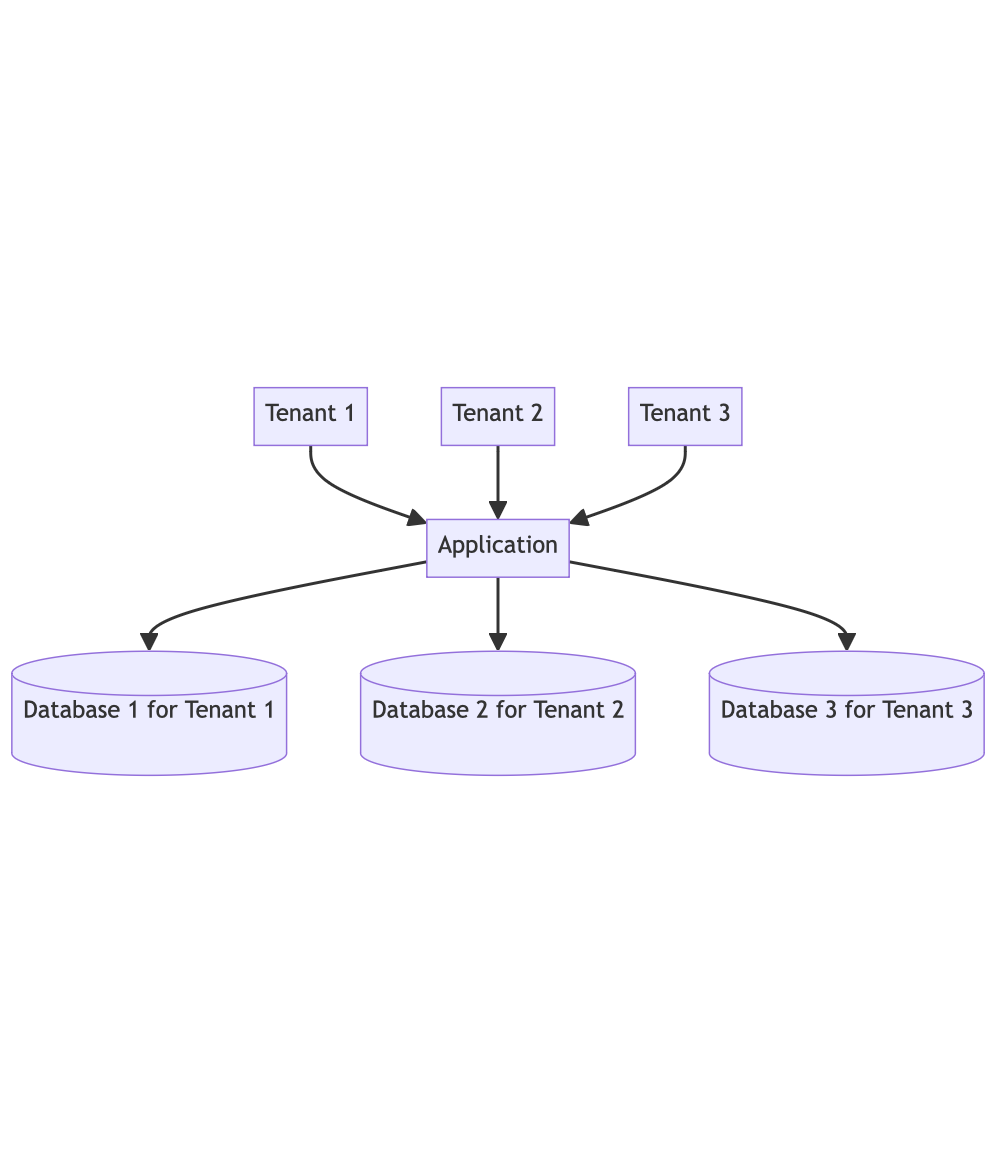
\includegraphics[width=80mm]{img/chap04/fig_multitenancy_multiple_databases.png}
\caption{Multi-tenancy with multiple databases}
\label{img04:multitenancy-multiple-databases}
\end{figure}

\subsubsection{Single database, multiple schemas}
%Each tenant has its own schema within a shared database, providing better data isolation while still sharing the same database instance.

This model involves a single database with multiple schemas, also referred to as "schema-level tenancy".
Each schema is serving a different tenant.
Infrastructure cost is significantly reduced compared to the previous approach, bringing some implementation complexities.


\begin{figure}[p]\centering
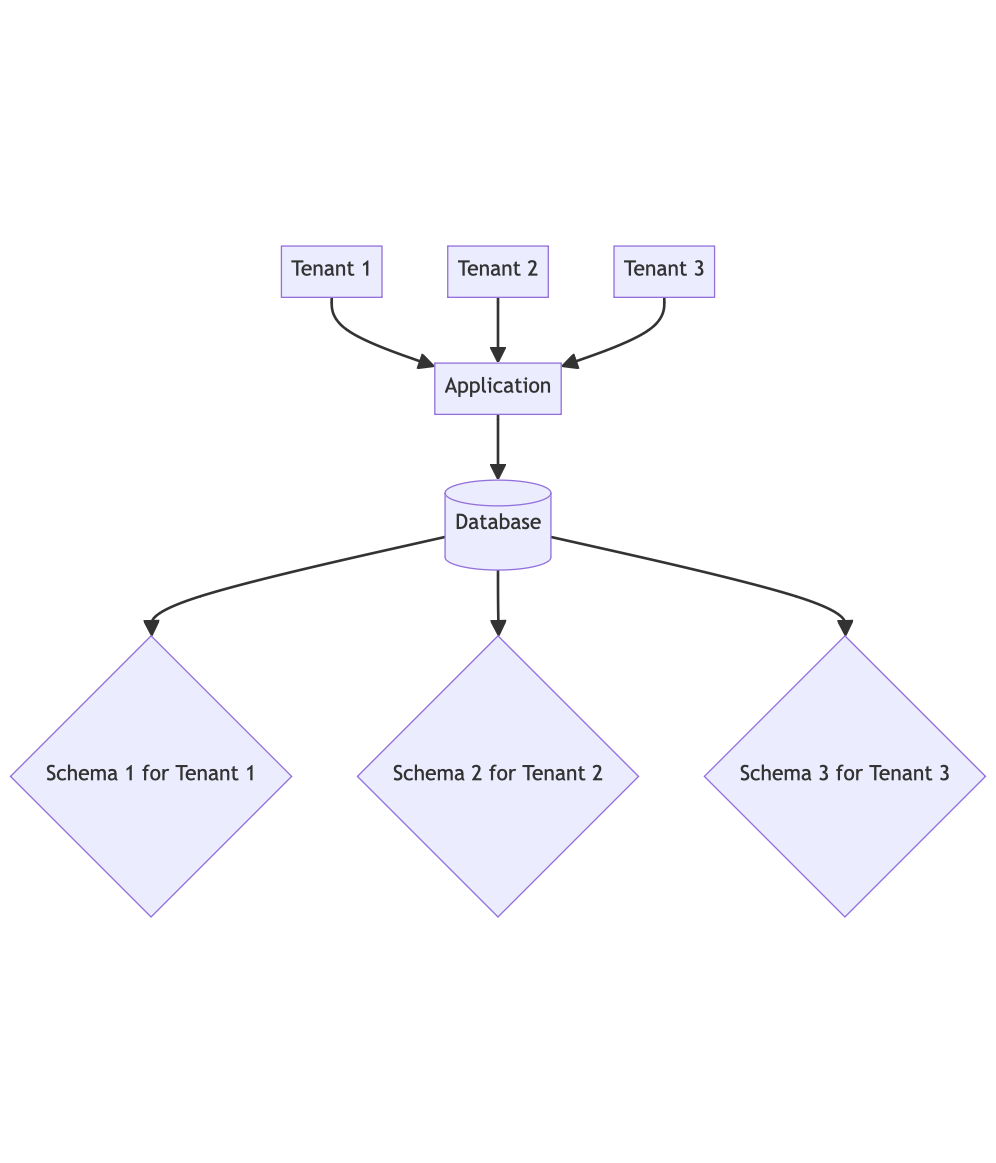
\includegraphics[width=80mm]{img/chap04/fig_multitenancy_multiple_schemas.png}
\caption{Multi-tenancy with multiple schemas}
\label{img04:multitenancy-multiple-schemas}
\end{figure}


\subsubsection{Single database, single schema}
\label{subsubsec:single-database-single-schema}
%Where all tenants share the same database and schema, but data is logically separated using tenant IDs in tables.
Known as "record level tenancy" is perhaps the most straight forward to implement.
All tenants share the same database and the same schema.
Tenant's data are stored in the same tables differentiated by column or columns containing a tenant identification.
This approach necessitates strict data isolation within application queries, as the application layer is the only enforcer of data separation.

\begin{figure}[p]\centering
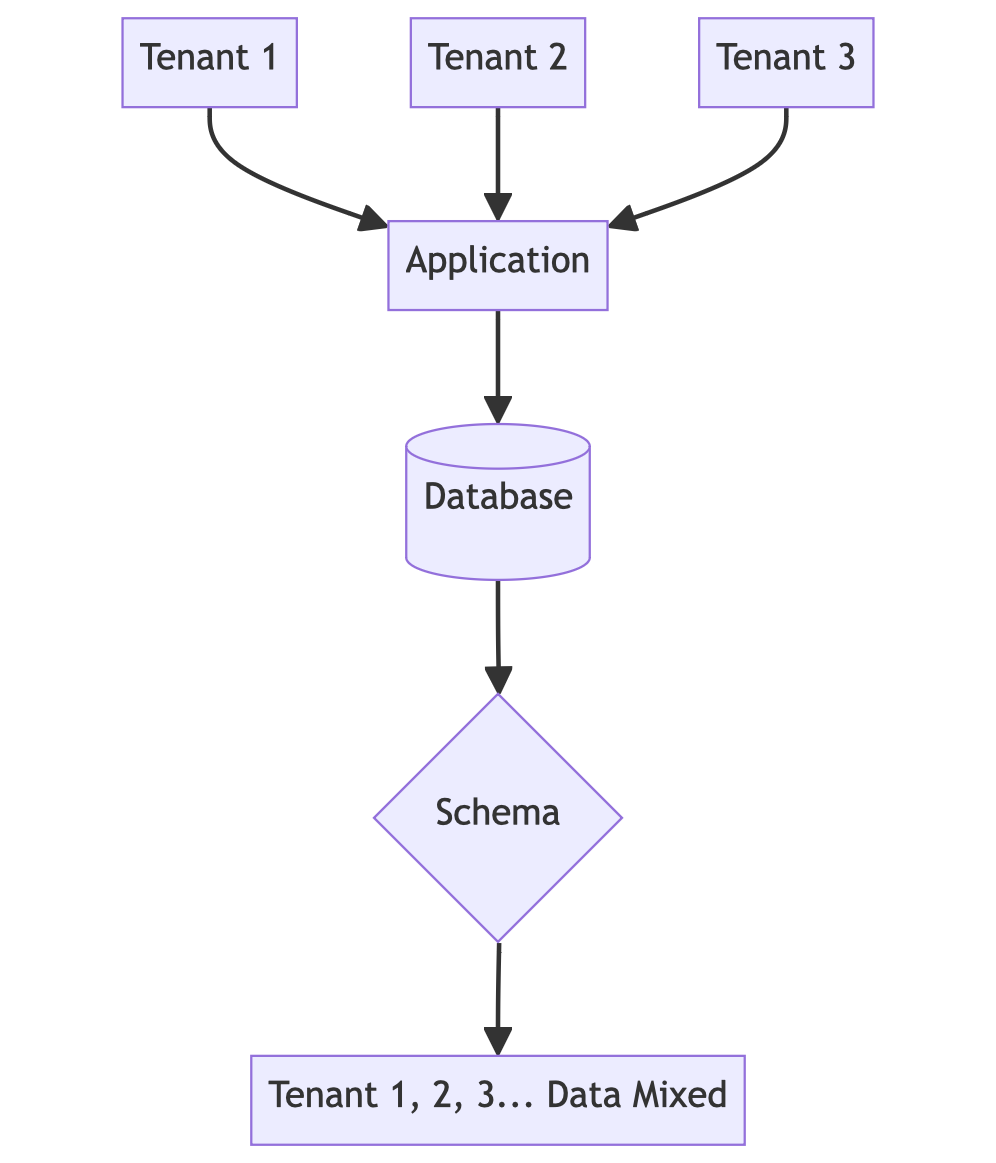
\includegraphics[width=80mm]{img/chap04/fig_multitenancy_single_database_single_schema.png}
\caption{Multi-tenancy with single database and schema}
\label{img04:multitenancy-single-database-single-schema}
\end{figure}


\subsection{Implementation in the platform}
% multitenancy is handled via so-called projects. Which are entities groupping multiple users sharing project biased entities between them with role based access
% data isolation is ensured via ORM queries which are project bias
The backend of the platform achieves multi-tenancy through the concepts of "Projects".
Projects are entities that bundle multiple users into a signle tenant, adopting the "record-level tenancy" seen in section \ref{subsubsec:single-database-single-schema}.

This setup allows users to share project-biased data among themselves with role-based access, ensuring that the data of each tenant are isolated and secure.
Without giving much detail that would compensate for the clarity of the design in figure \ref{img04:uml-user-project} we can see a simple UML diagram of the relation ship. 
Both \texttt{User} and \texttt{Project} have many more relations; however, these were removed for now.
Data isolation is ensured through ORM queries that are project-biased, thus preventing accidental data leaks between tenants.


%classDiagram
%    class Project {
%      +string id
%      +string name
%      +User owner
%      +User[] users
%    }

%    class User {
%      +string id
%      +string email
%      +string firstName
%      +string lastName
%      +string? planId
%      +Role? role
%    }

%    Project "1" -- "1" User : owner
%    Project "*" -- "*" User : users

\begin{figure}[p]\centering
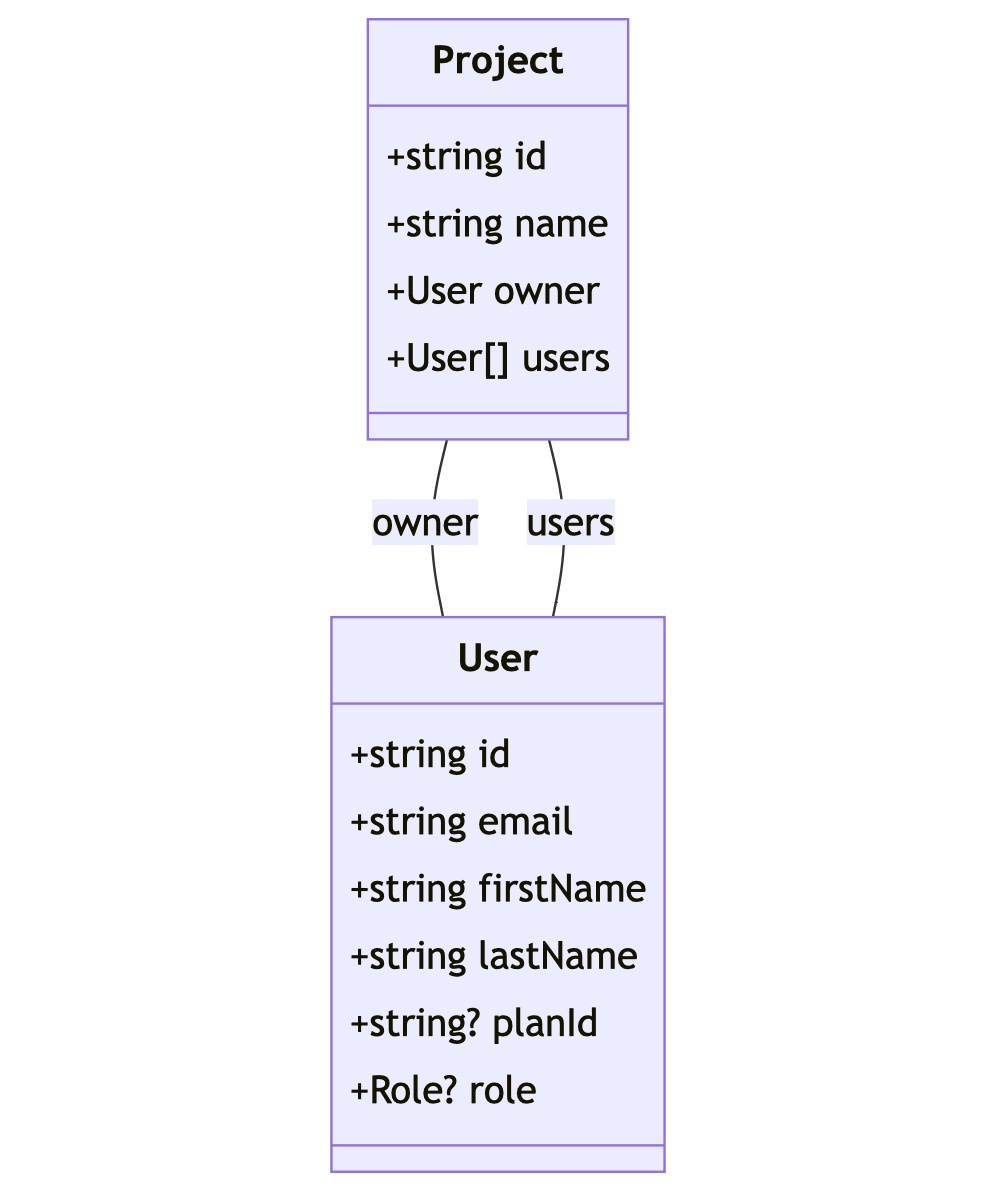
\includegraphics[width=140mm]{img/chap04/fig_simplified_project_concept.png}
\caption{Simplified UML diagram of the User and Project relation}
\label{img04:uml-user-project}
\end{figure}
